\chapter{Statistical Analysis Plots}
	\label{ap:stat}


	This appendix contains a closer look at the statistical analysis plots. Figures \ref{fig:LLR_CI_con} and \ref{fig:LLR_CI_des} show the LLR distributions for the constructive and destructive signals respectively with the prior $1/\Lambda^{2}$ and in figures \ref{fig:LLR_CI_con_4} and \ref{fig:LLR_CI_des_4} for the prior $1/\Lambda^{4}$. Figures \ref{fig:Theta_CI_con} and \ref{fig:Theta_CI_des} show the peudo-experiments distributions with expected and observed limits for constructive and destructive interference respectively with a $1/\Lambda^{2}$ prior and in figures \ref{fig:Theta_CI_con_4} and \ref{fig:Theta_CI_des_4} for the prior $1/\Lambda^{4}$. 

	% \begin{figure}[h]
	% 	\centering
	% 		\includegraphics[width=0.9\linewidth]{images/}
	% 	\caption{}
	% 	\label{fig:}
	% \end{figure}



    \begin{figure}[h]
        \begin{center}
            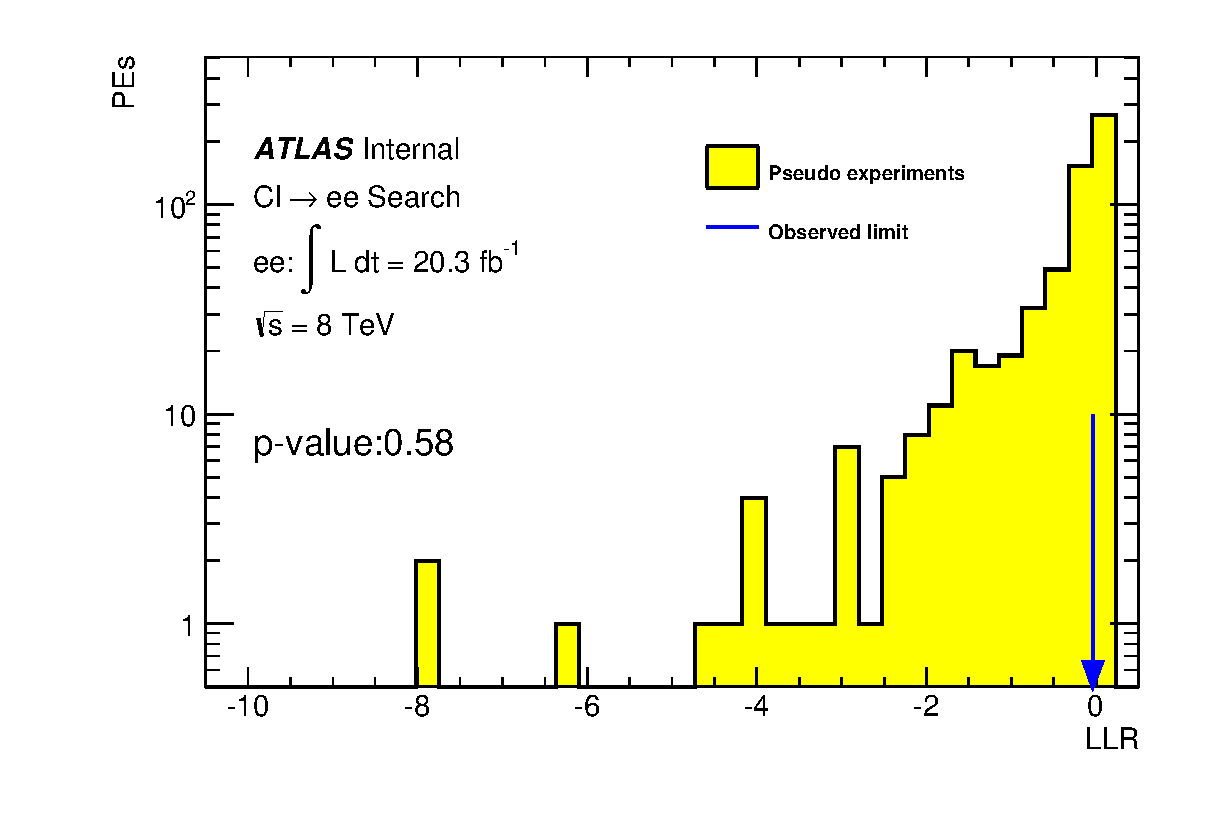
\includegraphics[width=0.42\linewidth]{images/ee__LL_minus_L2/LLR.eps}
            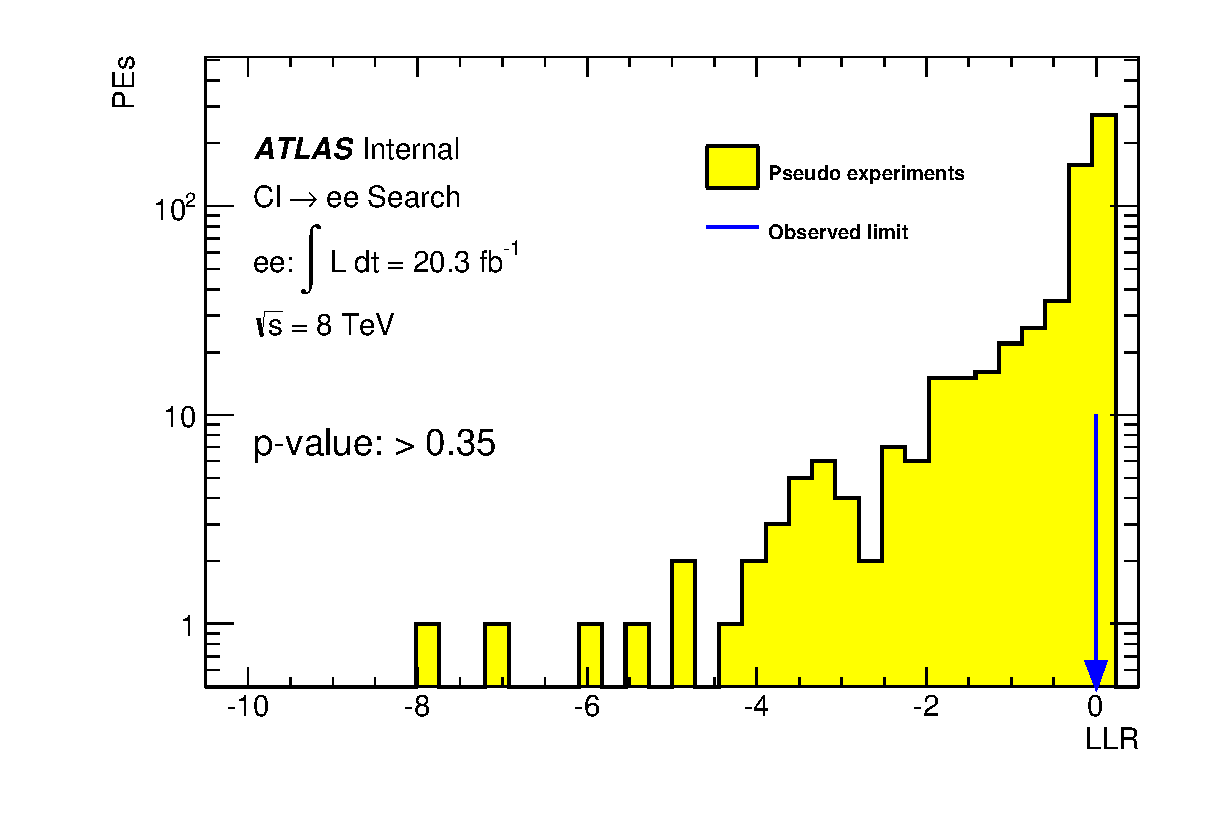
\includegraphics[width=0.42\linewidth]{images/ee__RR_minus_L2/LLR.eps}
            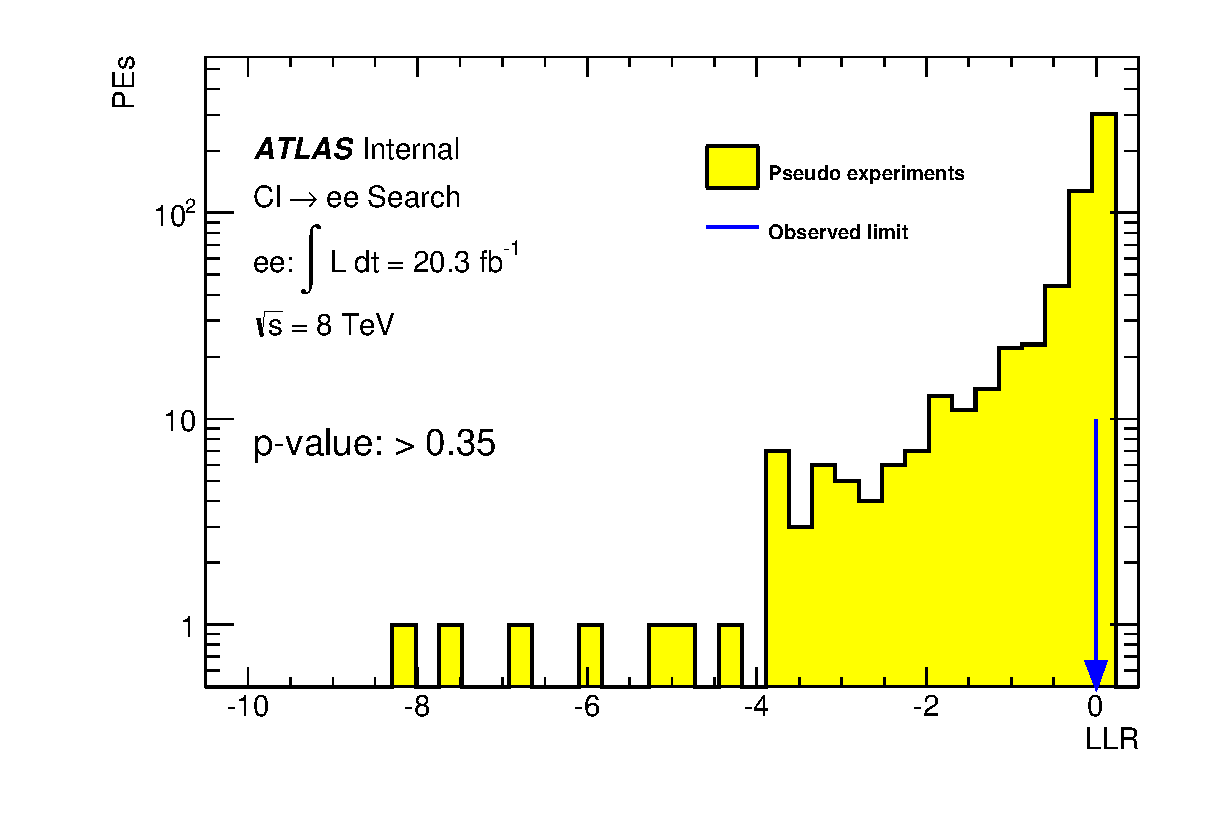
\includegraphics[width=0.42\linewidth]{images/ee__LR_minus_L2/LLR.eps}
        \end{center}
       \caption{Distribution of negative Log Likelihood Ratio's for the CI formalisms LL (top left), RR (top right) and LR (bottom) with constructive interference given a uniform positive prior in $1/\Lambda^{2}$.}
       \label{fig:LLR_CI_con}
    \end{figure}



    \begin{figure}[h]
        \begin{center}
            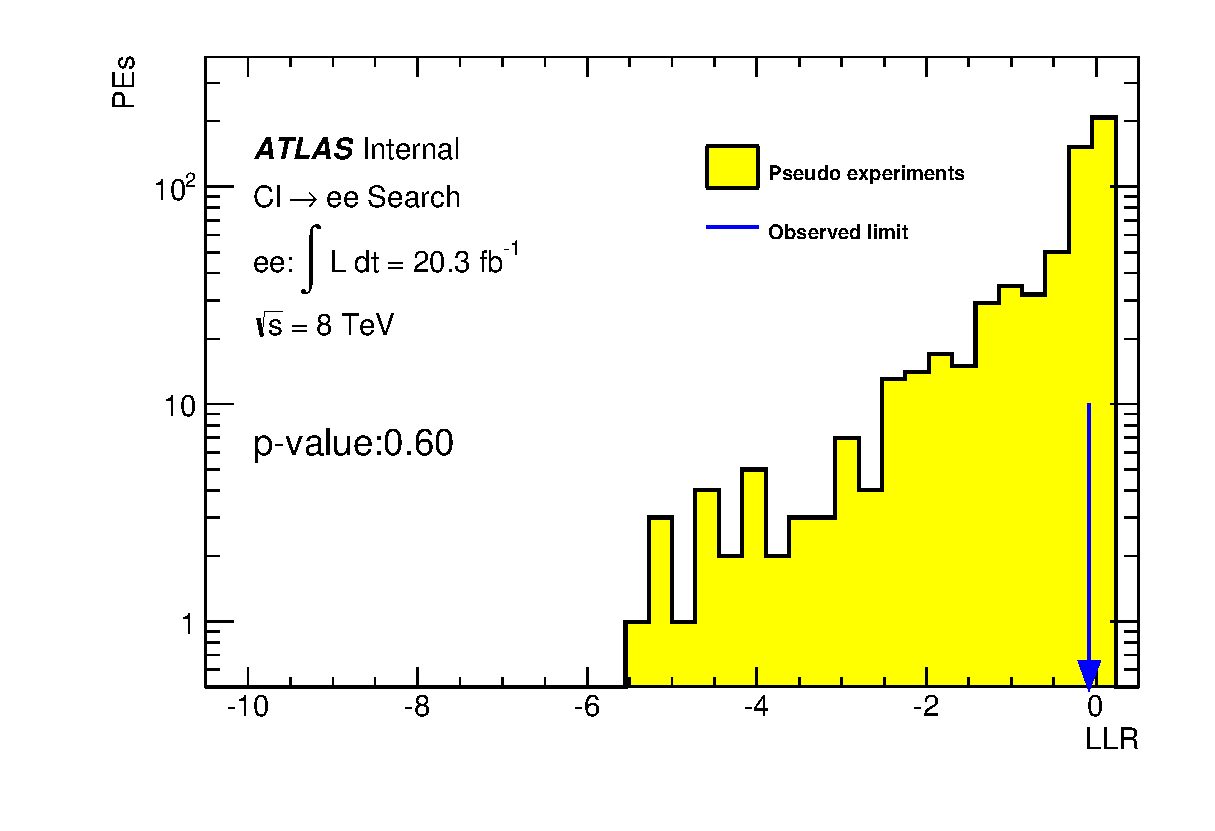
\includegraphics[width=0.42\linewidth]{images/ee__LL_plus_L2/LLR.eps}
            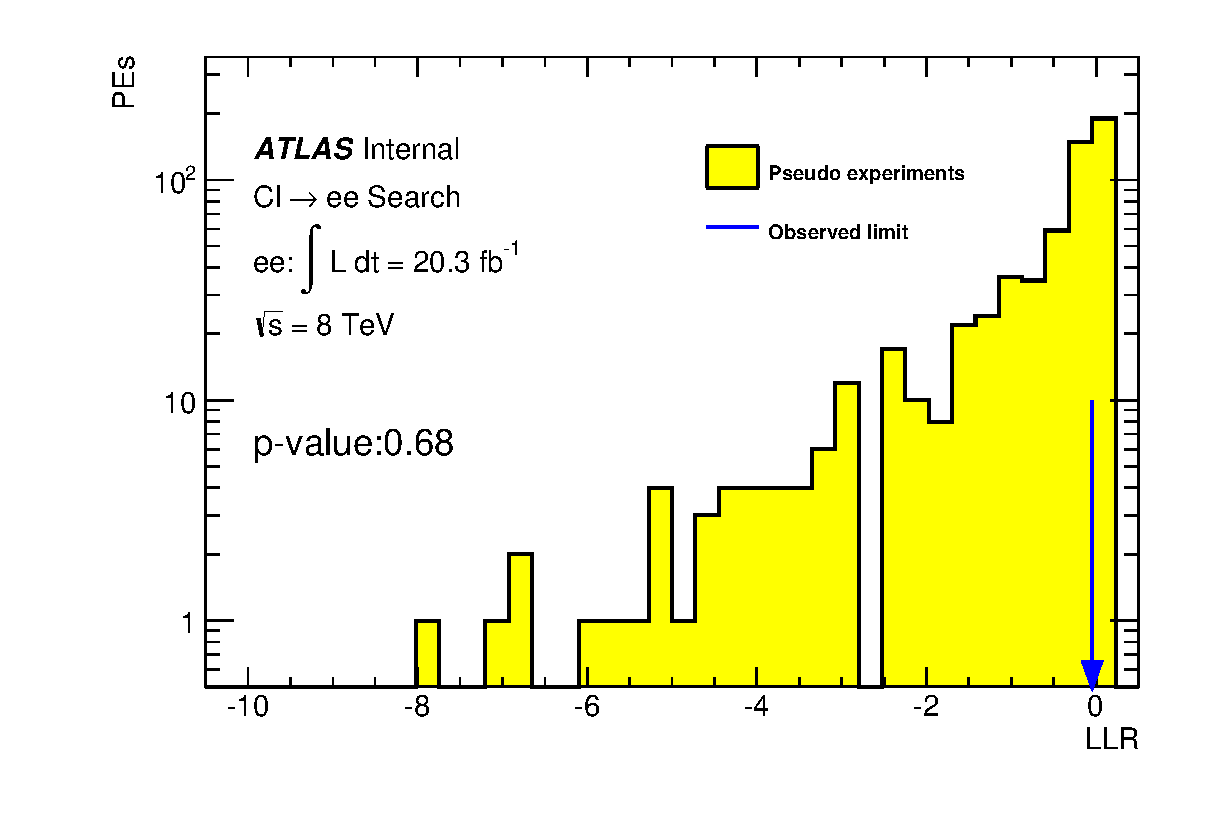
\includegraphics[width=0.42\linewidth]{images/ee__RR_plus_L2/LLR.eps}
            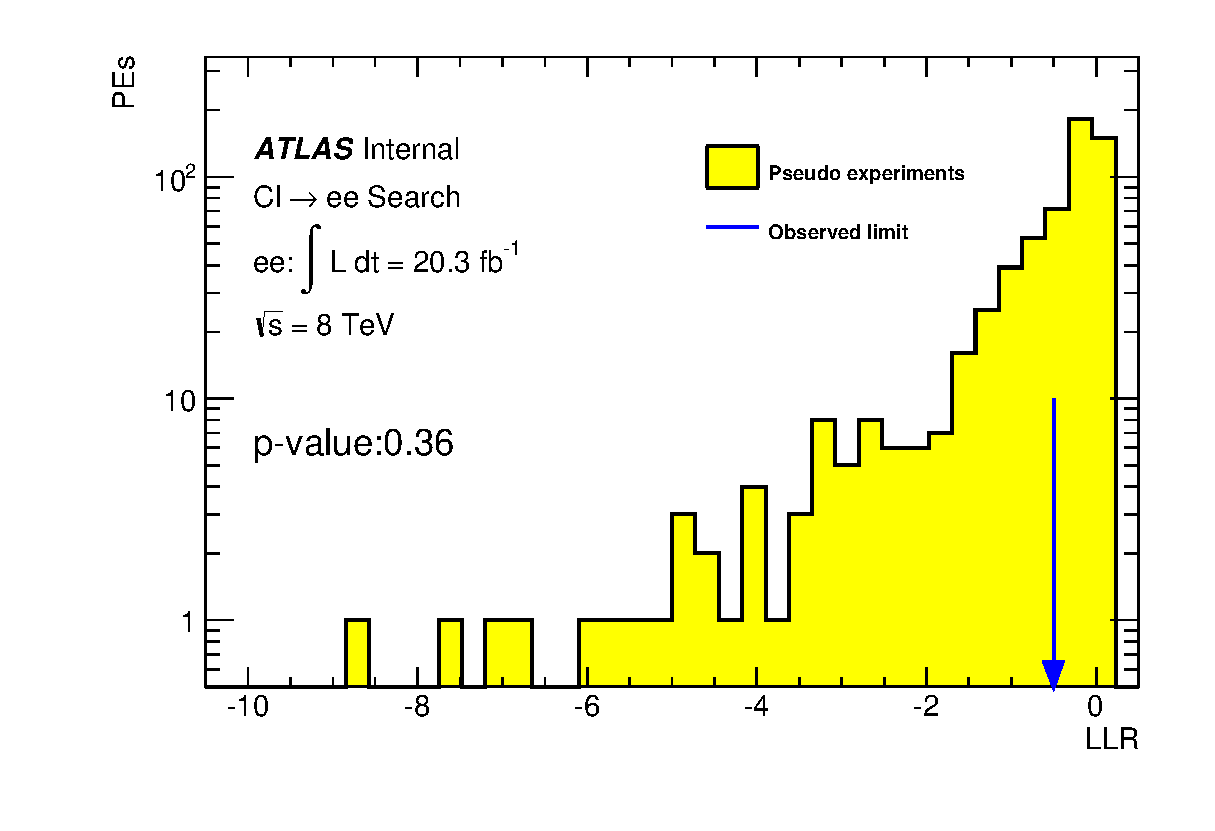
\includegraphics[width=0.42\linewidth]{images/ee__LR_plus_L2/LLR.eps}
        \end{center}
       \caption{Distribution of negative Log Likelihood Ratio's for the CI formalisms LL (top left), RR (top right) and LR (bottom) with destructive interference given a uniform positive prior in $1/\Lambda^{2}$.}
       \label{fig:LLR_CI_des}
    \end{figure}



       \begin{figure}[h]
        \begin{center}
            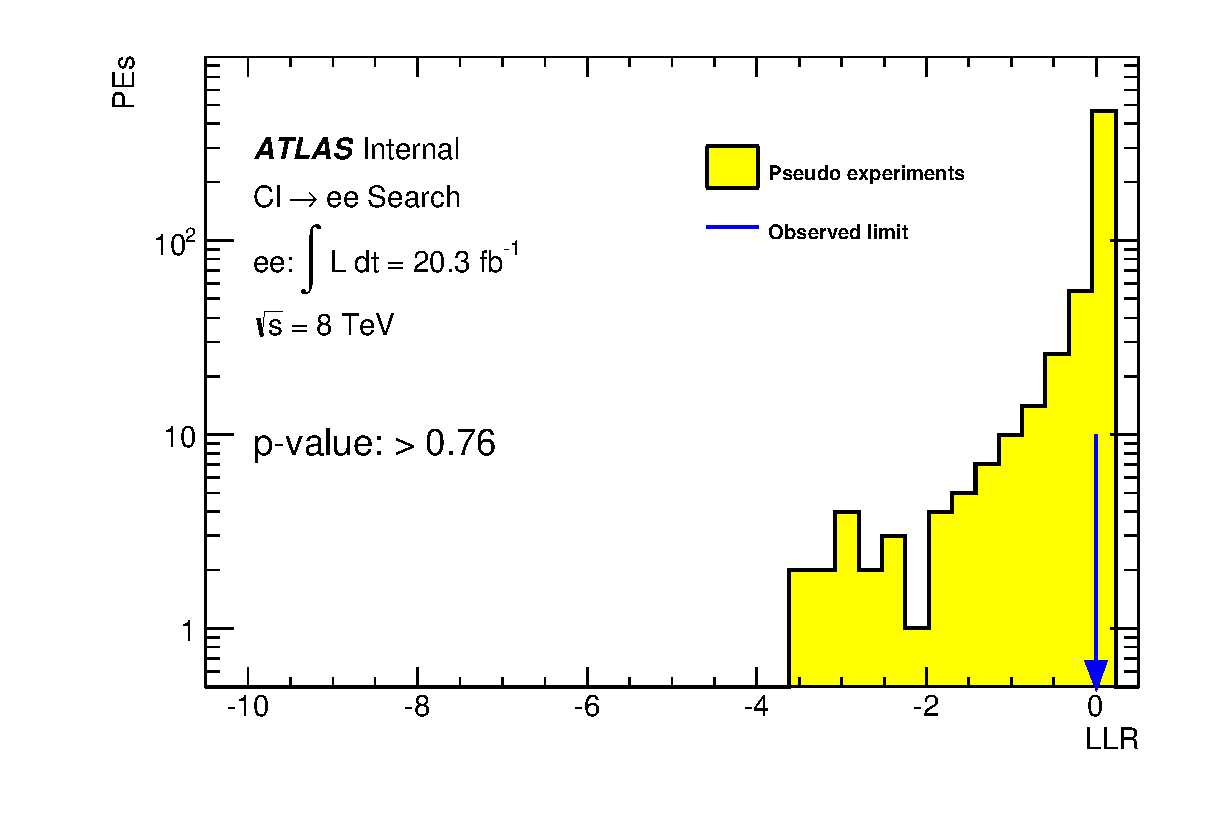
\includegraphics[width=0.42\linewidth]{images/ee__LL_minus_L4/LLR.eps}
            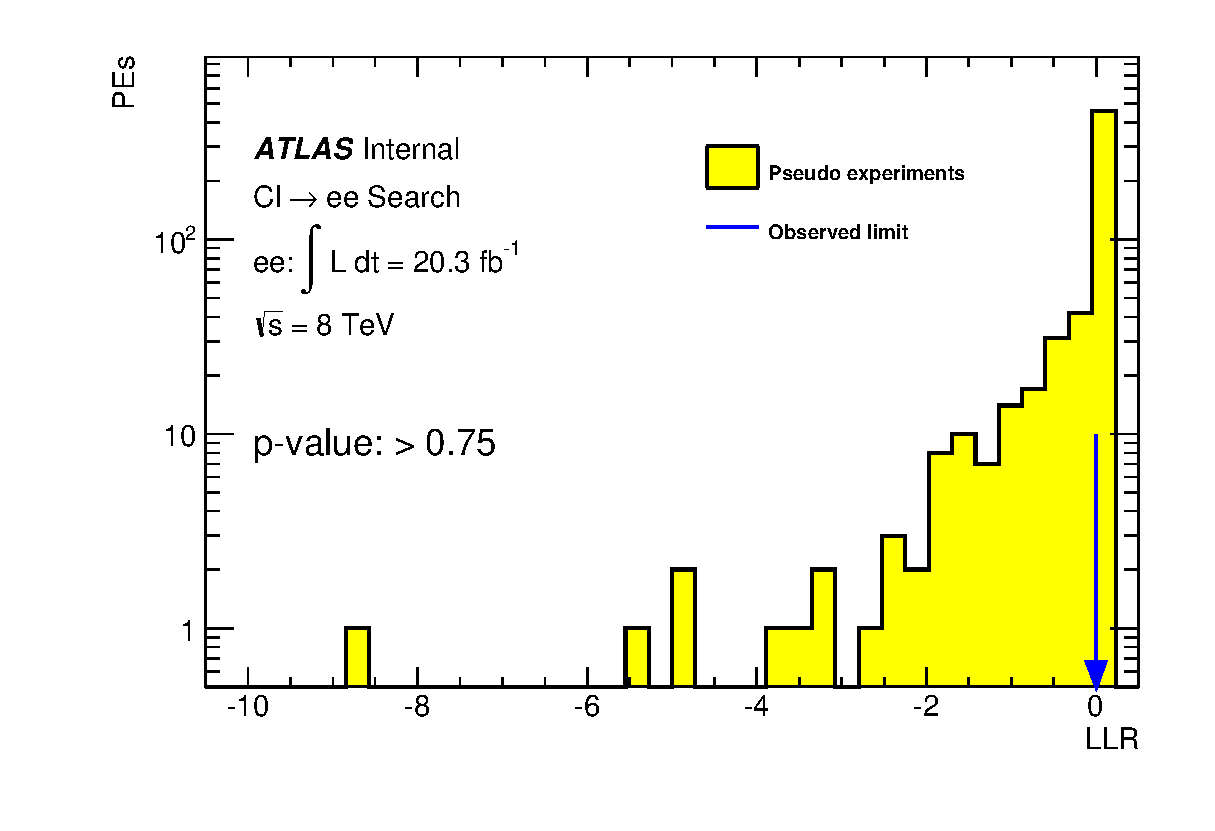
\includegraphics[width=0.42\linewidth]{images/ee__RR_minus_L4/LLR.eps}
            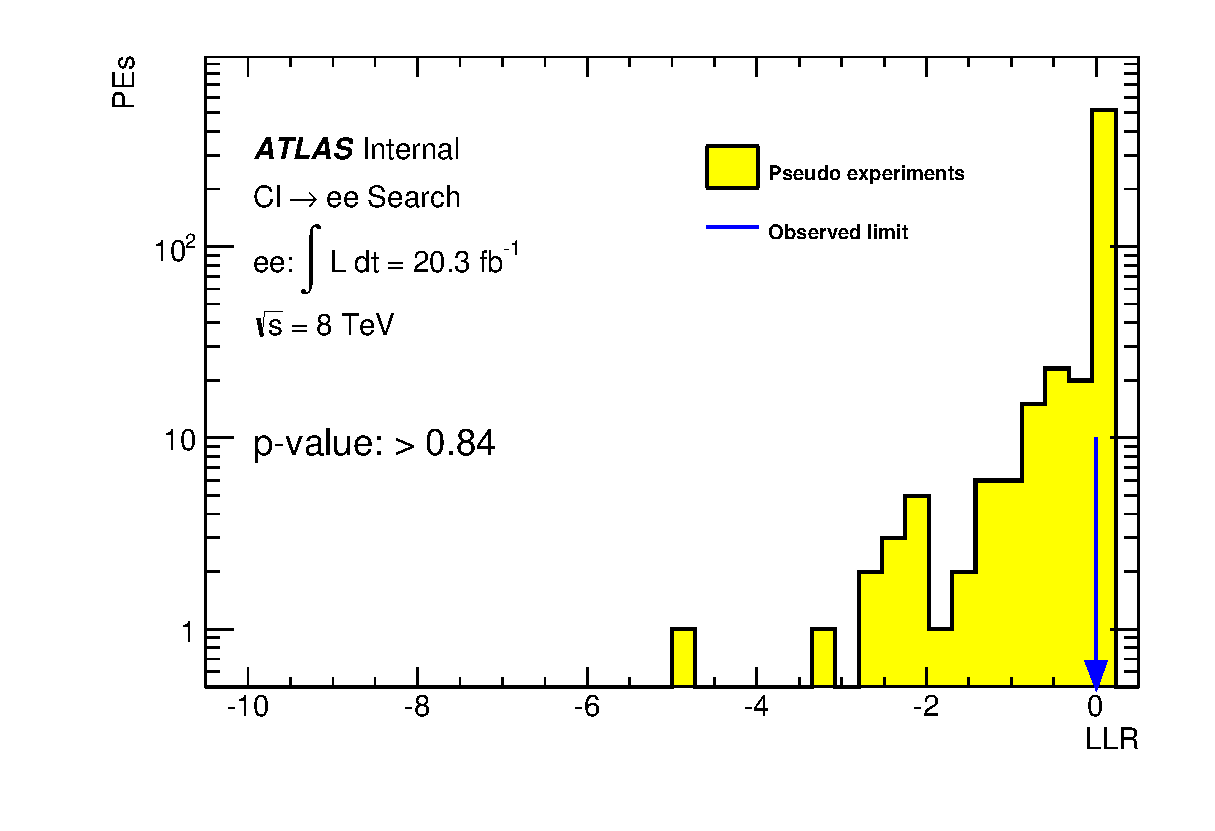
\includegraphics[width=0.42\linewidth]{images/ee__LR_minus_L4/LLR.eps}
        \end{center}
       \caption{Distribution of negative Log Likelihood Ratio's for the CI formalisms LL (top left), RR (top right) and LR (bottom) with constructive interference given a uniform positive prior in $1/\Lambda^{4}$.}
       \label{fig:LLR_CI_con_4}
    \end{figure}



    \begin{figure}[h]
        \begin{center}
            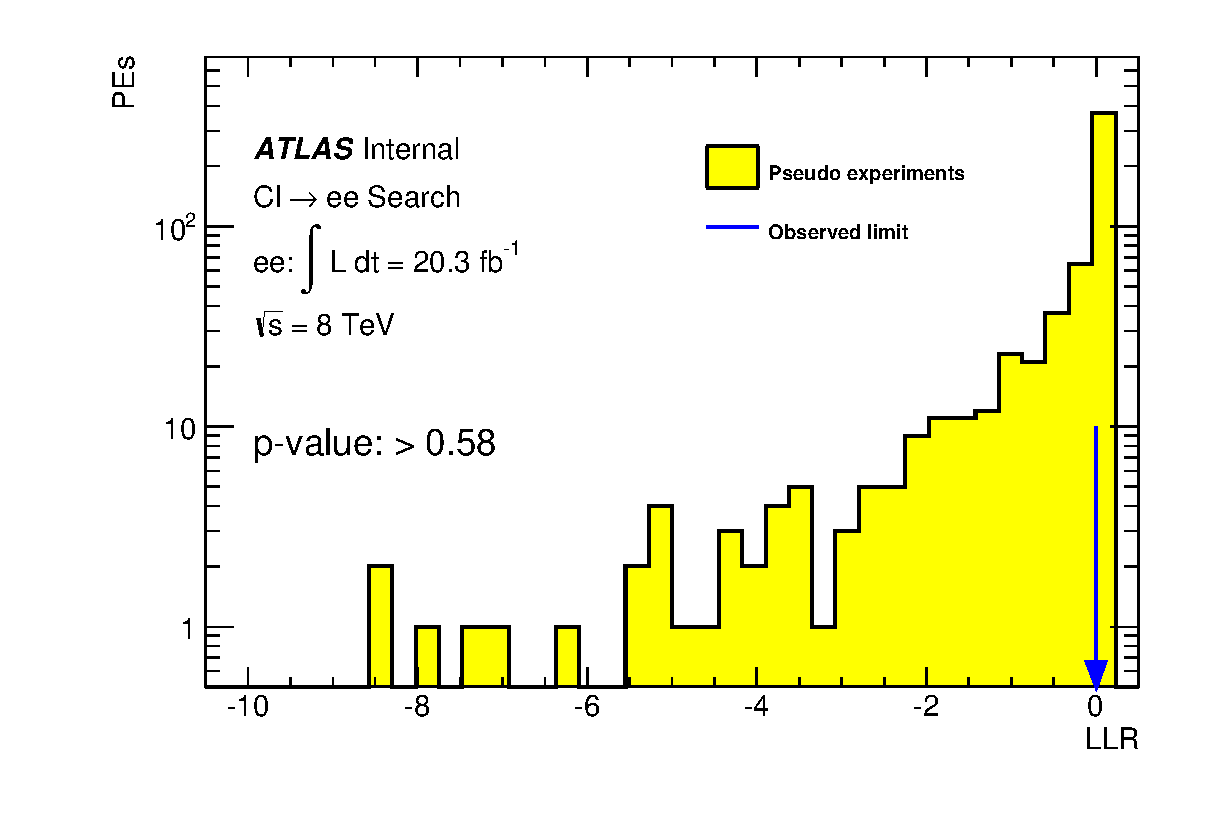
\includegraphics[width=0.42\linewidth]{images/ee__LL_plus_L4/LLR.eps}
            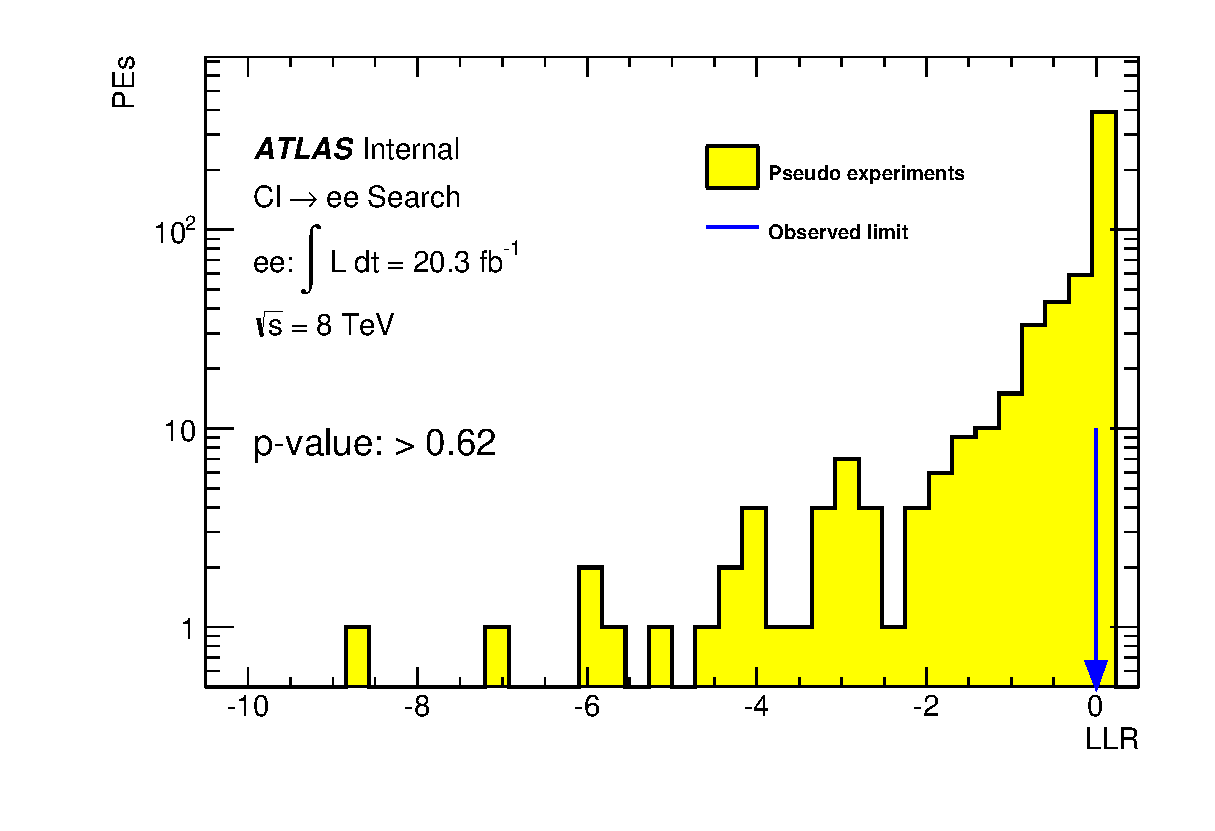
\includegraphics[width=0.42\linewidth]{images/ee__RR_plus_L4/LLR.eps}
            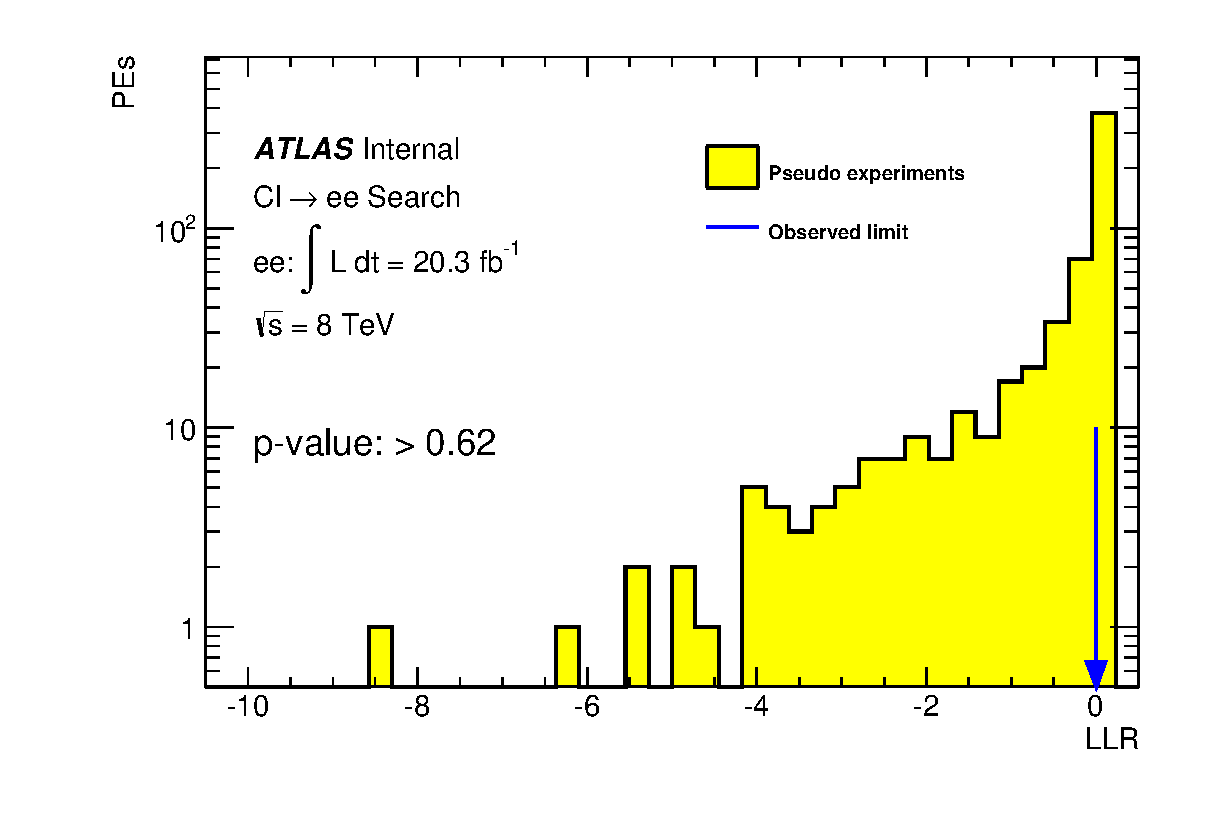
\includegraphics[width=0.42\linewidth]{images/ee__LR_plus_L4/LLR.eps}
        \end{center}
       \caption{Distribution of negative Log Likelihood Ratio's for the CI formalisms LL (top left), RR (top right) and LR (bottom) with destructive interference given a uniform positive prior in $1/\Lambda^{4}$.}
       \label{fig:LLR_CI_des_4}
    \end{figure}
















    \begin{figure}[h]
        \begin{center}
            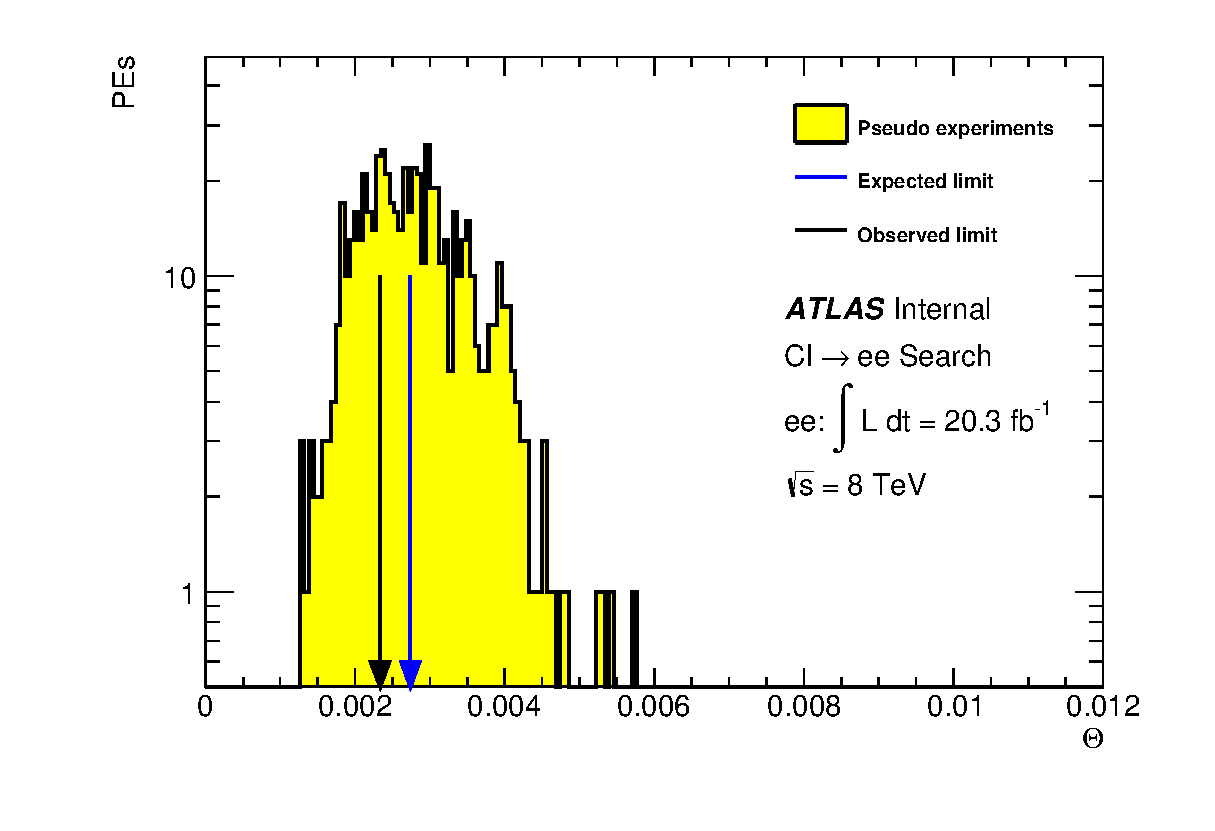
\includegraphics[width=0.7\linewidth]{images/ee__LL_minus_L2/Theta.eps}
            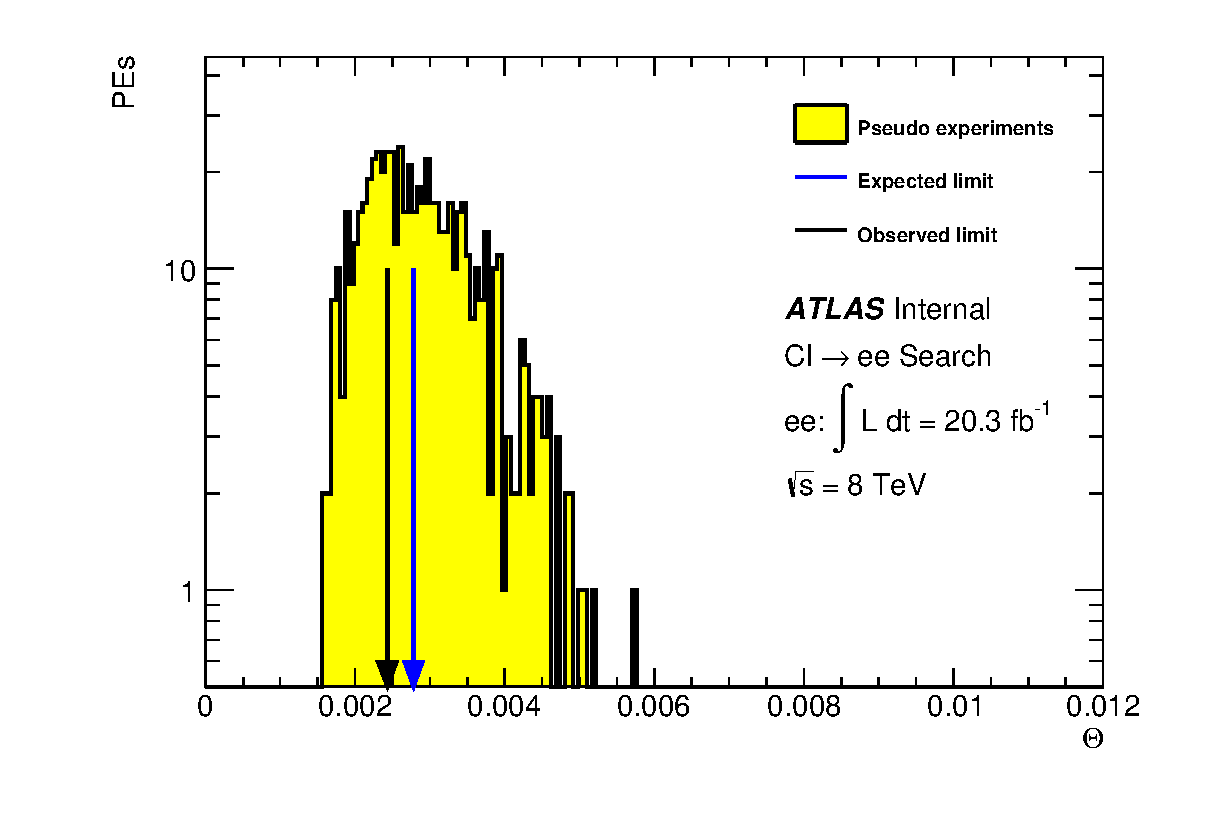
\includegraphics[width=0.7\linewidth]{images/ee__RR_minus_L2/Theta.eps}
            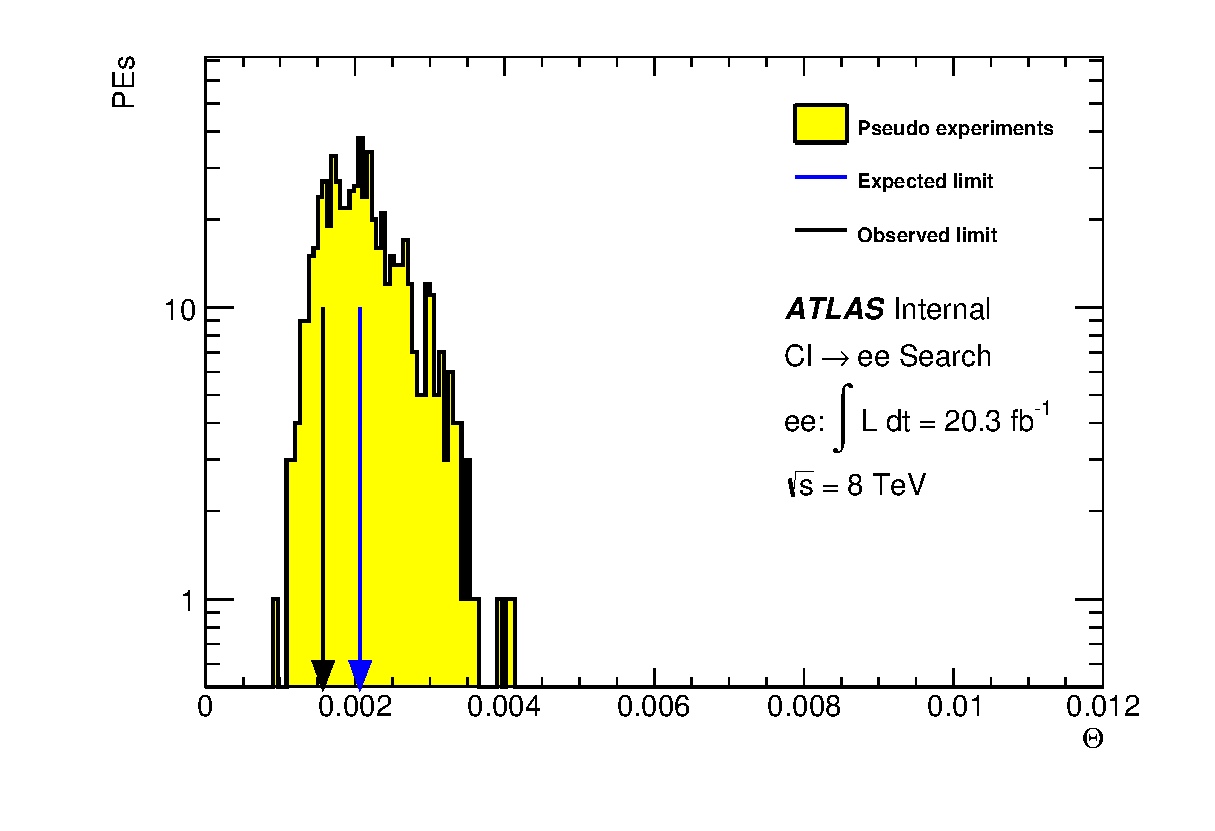
\includegraphics[width=0.7\linewidth]{images/ee__LR_minus_L2/Theta.eps}
        \end{center}
       \caption{Distribution of PE's with associated limits for CI formalisms LL (top left), RR (top right) and LR (bottom) with constructive interference given a uniform positive prior in $1/\Lambda^{2}$. The mean value is shown as the expected limit for comparison to the observed limit shown. $\Theta$ = $1/\Lambda^{2}$}
       \label{fig:Theta_CI_con}
    \end{figure}


    \begin{figure}[h]
        \begin{center}
            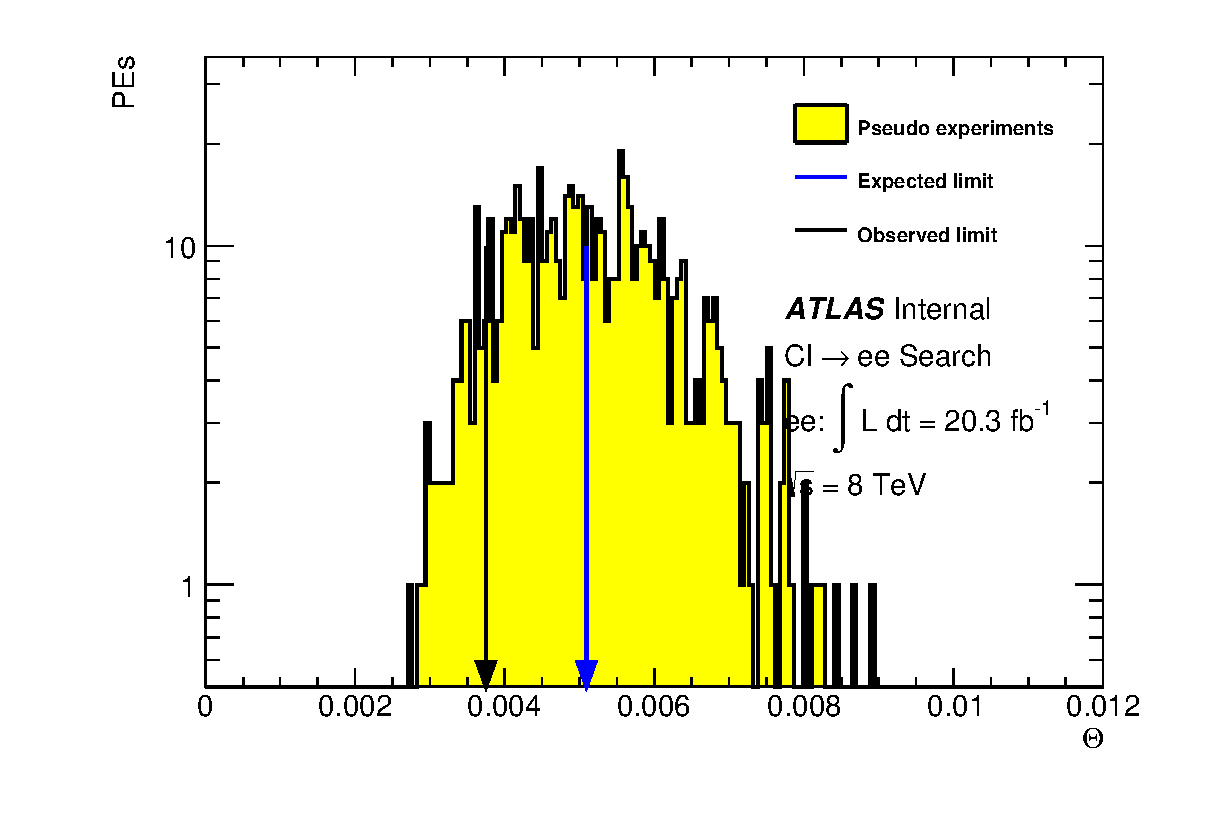
\includegraphics[width=0.7\linewidth]{images/ee__LL_plus_L2/Theta.eps}
            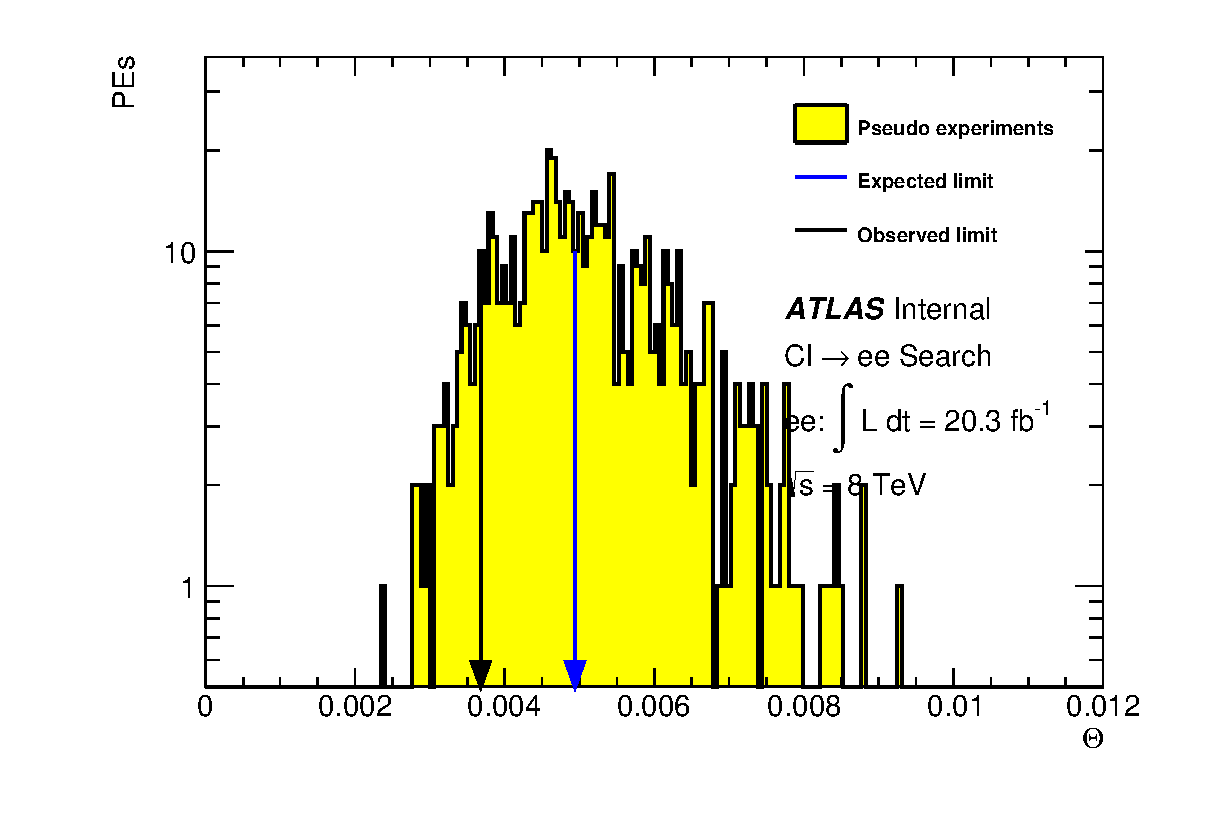
\includegraphics[width=0.7\linewidth]{images/ee__RR_plus_L2/Theta.eps}
            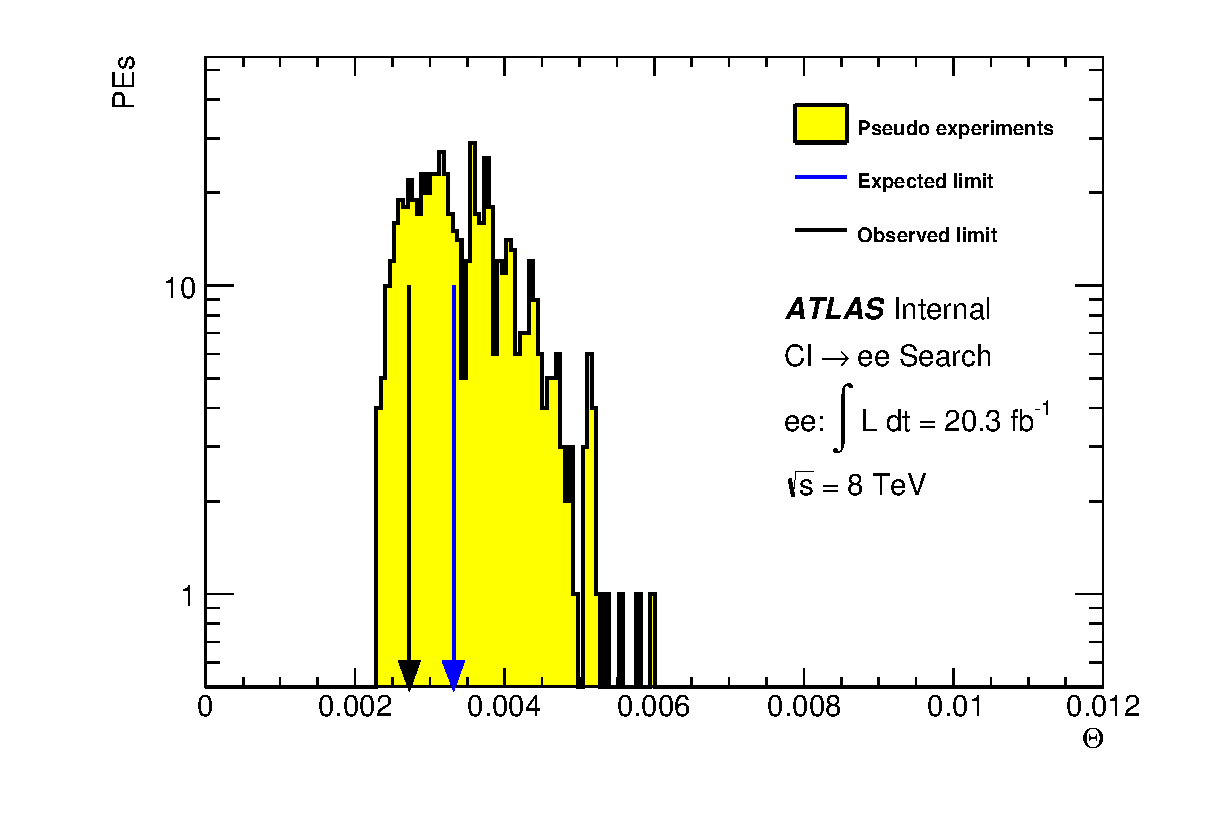
\includegraphics[width=0.7\linewidth]{images/ee__LR_plus_L2/Theta.eps}
        \end{center}
       \caption{Distribution of PE's with associated limits for CI formalisms LL (top left), RR (top right) and LR (bottom) with destructive interference given a uniform positive prior in $1/\Lambda^{2}$. The mean value is shown as the expected limit for comparison to the observed limit shown. $\Theta$ = $1/\Lambda^{2}$}
       \label{fig:Theta_CI_des}
    \end{figure}



    \begin{figure}[h]
        \begin{center}
            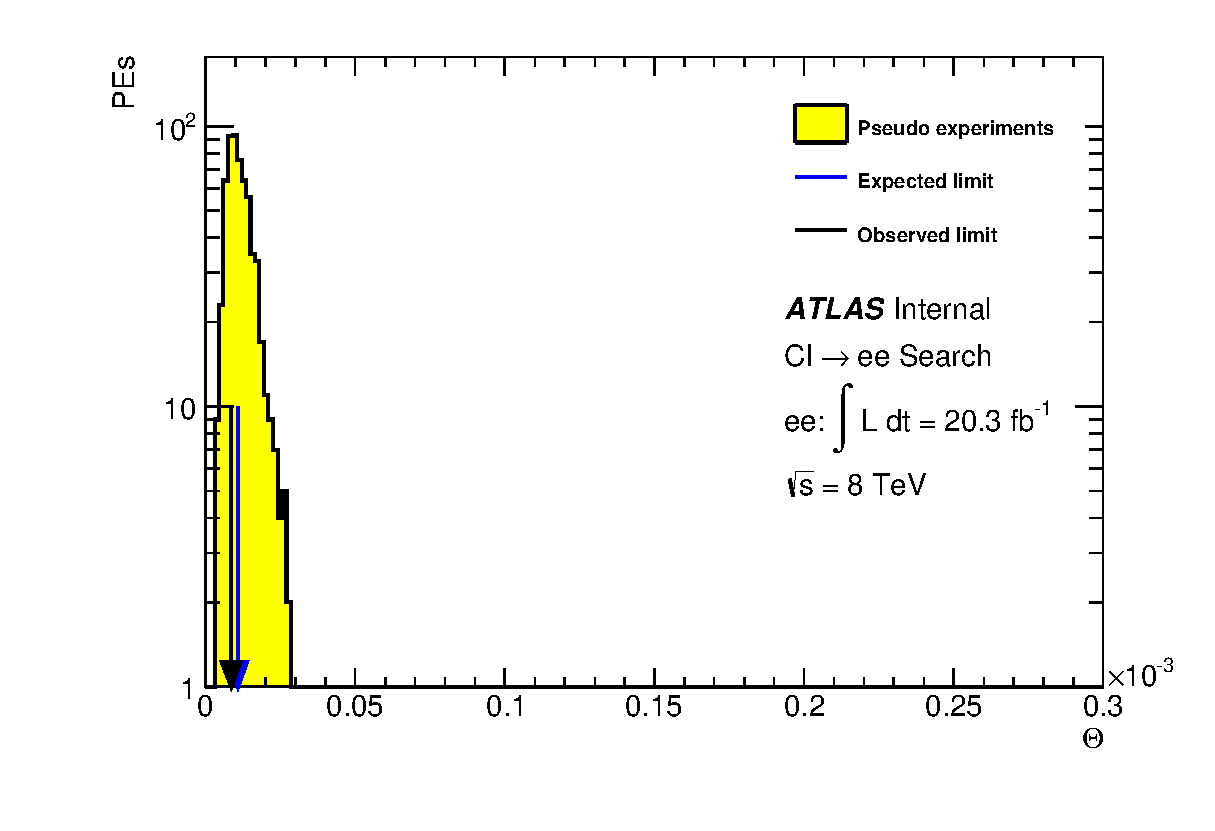
\includegraphics[width=0.7\linewidth]{images/ee__LL_minus_L4/Theta.eps}
            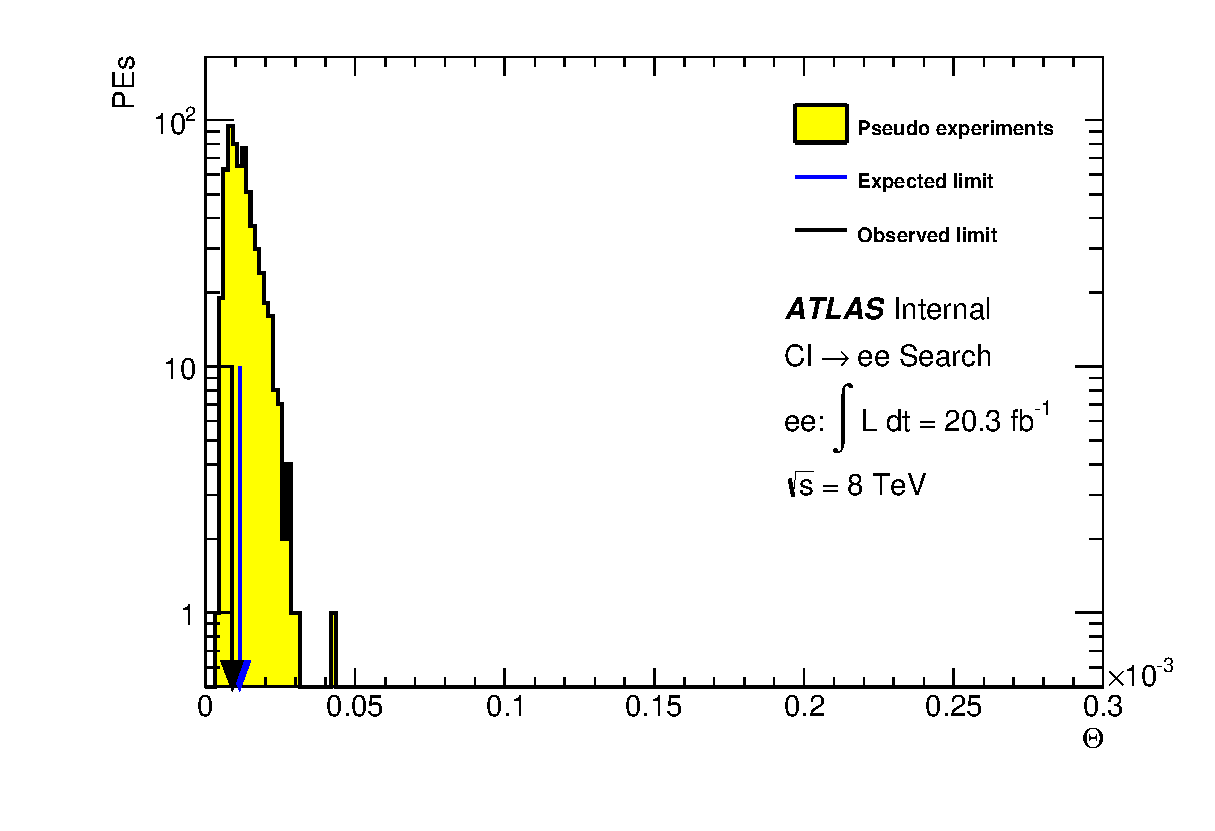
\includegraphics[width=0.7\linewidth]{images/ee__RR_minus_L4/Theta.eps}
            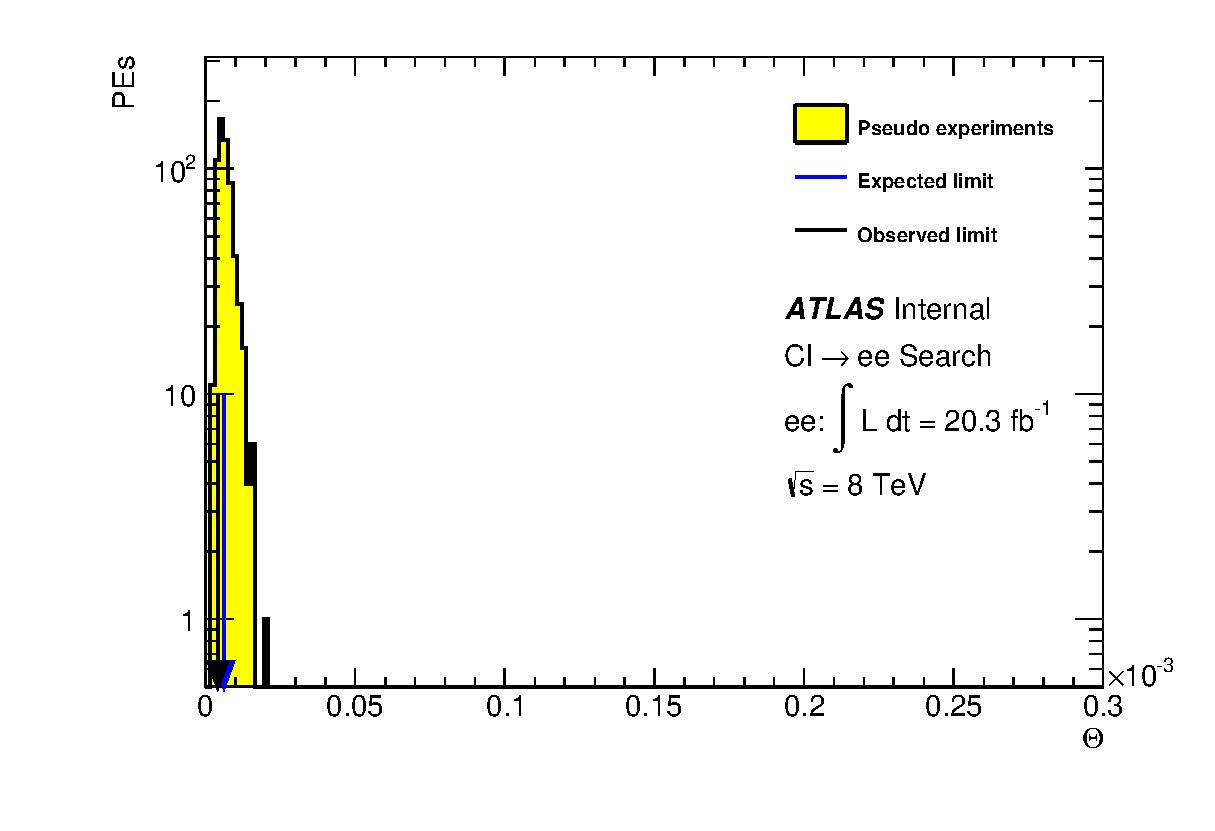
\includegraphics[width=0.7\linewidth]{images/ee__LR_minus_L4/Theta.eps}
        \end{center}
       \caption{Distribution of PE's with associated limits for CI formalisms LL (top left), RR (top right) and LR (bottom) with constructive interference given a uniform positive prior in $1/\Lambda^{4}$. The mean value is shown as the expected limit for comparison to the observed limit shown. $\Theta$ = $1/\Lambda^{4}$}
       \label{fig:Theta_CI_con_4}
    \end{figure}


    \begin{figure}[h]
        \begin{center}
            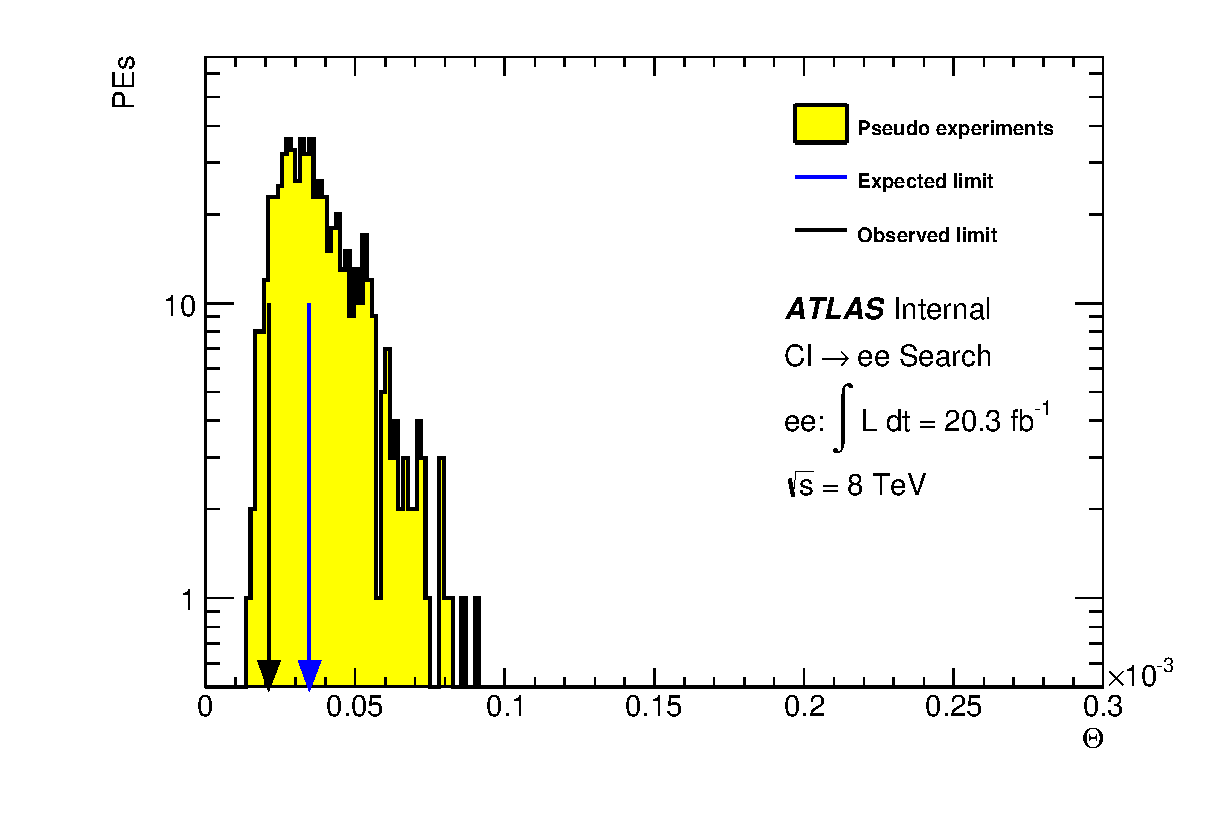
\includegraphics[width=0.7\linewidth]{images/ee__LL_plus_L4/Theta.eps}
            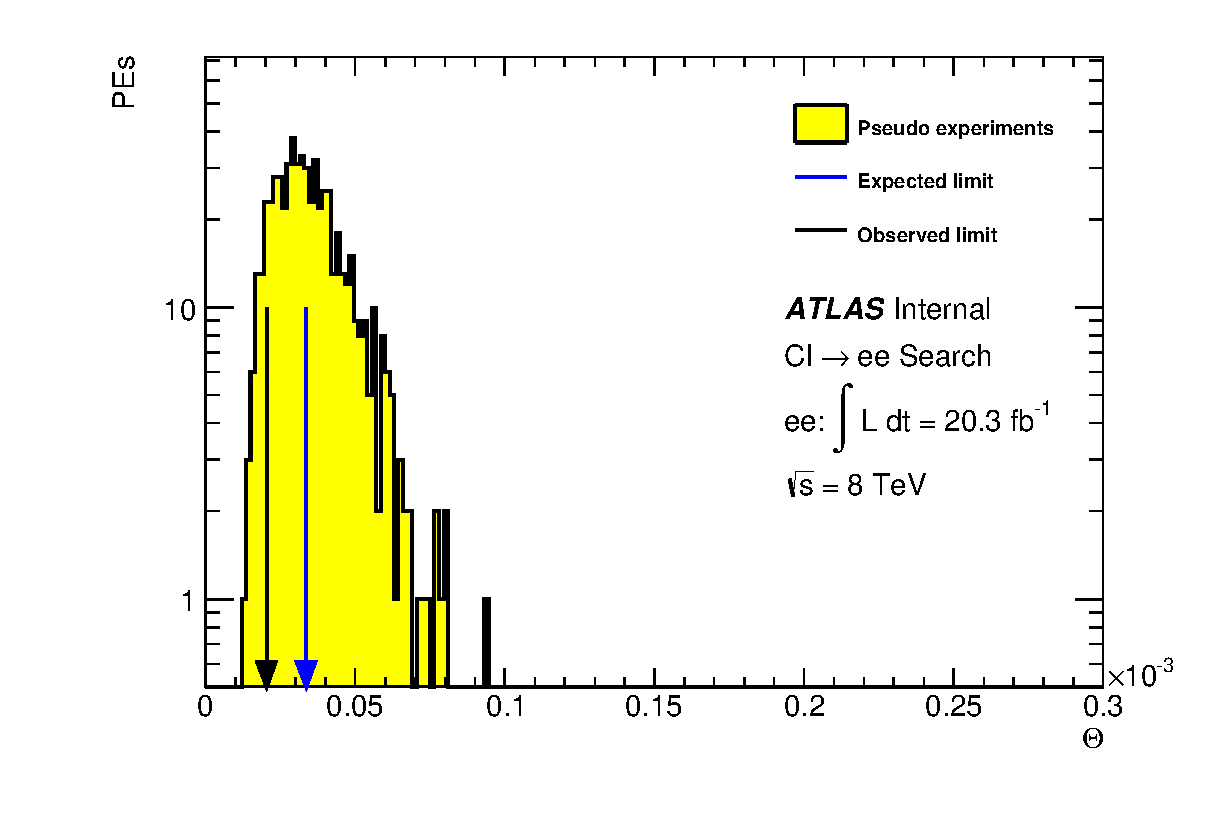
\includegraphics[width=0.7\linewidth]{images/ee__RR_plus_L4/Theta.eps}
            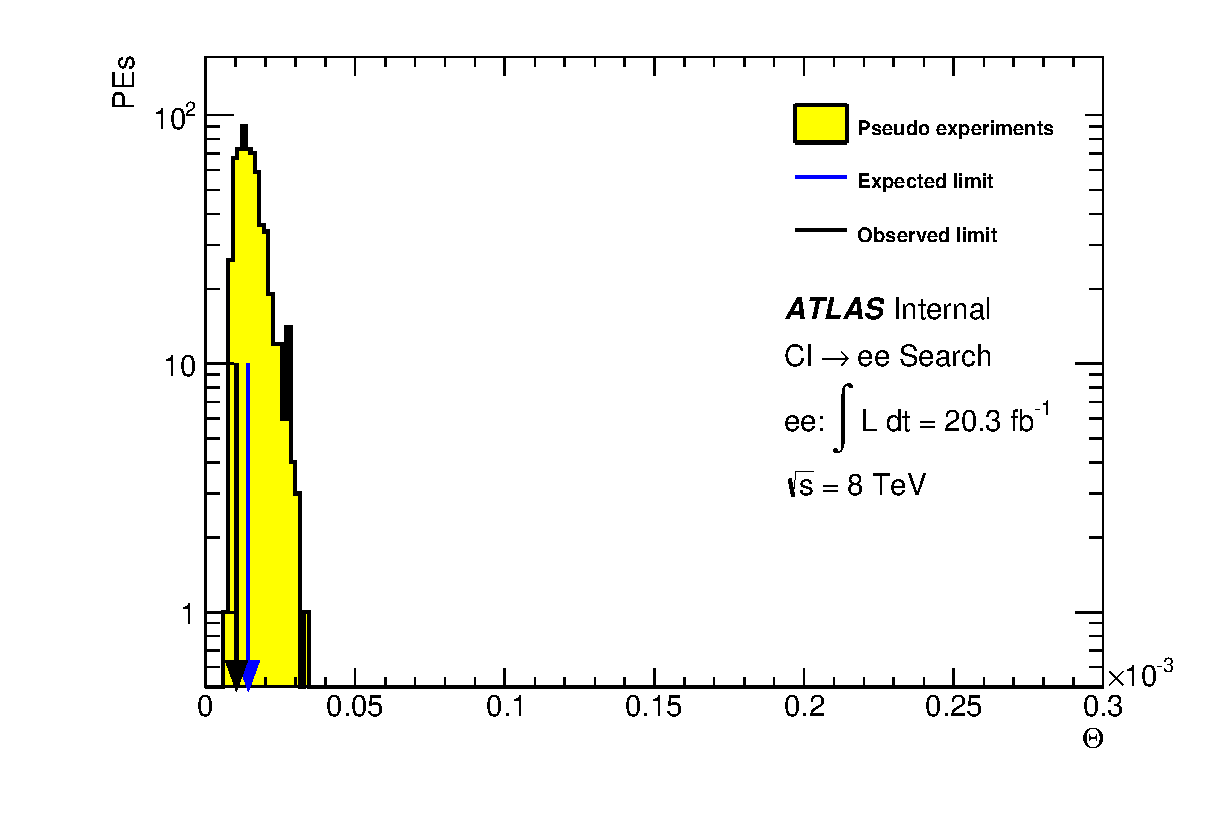
\includegraphics[width=0.7\linewidth]{images/ee__LR_plus_L4/Theta.eps}
        \end{center}
       \caption{Distribution of PE's with associated limits for CI formalisms LL (top left), RR (top right) and LR (bottom) with destructive interference given a uniform positive prior in $1/\Lambda^{4}$. The mean value is shown as the expected limit for comparison to the observed limit shown. $\Theta$ = $1/\Lambda^{4}$}
       \label{fig:Theta_CI_des_4}
    \end{figure}








